\documentclass{beamer}

\usepackage{beamerthemesplit}
\usepackage{latexsym}
\usepackage{eurosym}
\usepackage[activeacute,spanish]{babel}
\usepackage{ae,aecompl}
\usepackage{graphicx}
\usepackage{amsfonts}

\usetheme{Darmstadt}

\title{Presentacion Proyecto Cinema}
\author{G. Chavez - K. Campuzano - J. Camacho - K. Altamirano}
\date{\today}

\begin{document}

\frame{\titlepage}

\section[Indice]{}
\begin{frame}[allowframebreaks]
\tableofcontents
\end{frame}
%\frame{\tableofcontents}

\section{Descripcion del Proyecto}
\begin{frame}[allowframebreaks]
\frametitle{Descripcion}
Cinema es una aplicacion movil complementaria al sistema de compra de snacks de un cine.\\

El cliente para ser atendido debera ingresar a la aplicacion y seguir los pasos para realizar el pedido,y el total se le descontara del saldo inicial del usuario.\\

Un elemento importante para realizar el pedido de comida es que el usuario ya haya comprado
sus entradas de cine, esto facilita al momento de entregarle el pedido al usuario.\\

\end{frame}





\section{Escenario de compra}
\begin{frame}[allowframebreaks]
\frametitle{Login}
\begin{figure}[h]
\centering
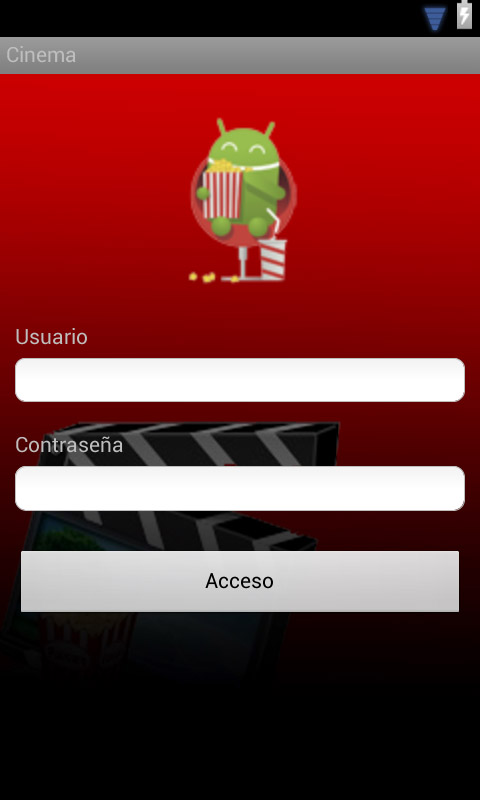
\includegraphics[height=0.8\textheight]{acceso.jpg}
\end{figure}
\end{frame}

\begin{frame}[allowframbreaks]
\frametitle{Menu Principal}
\begin{figure}[h]
\centering
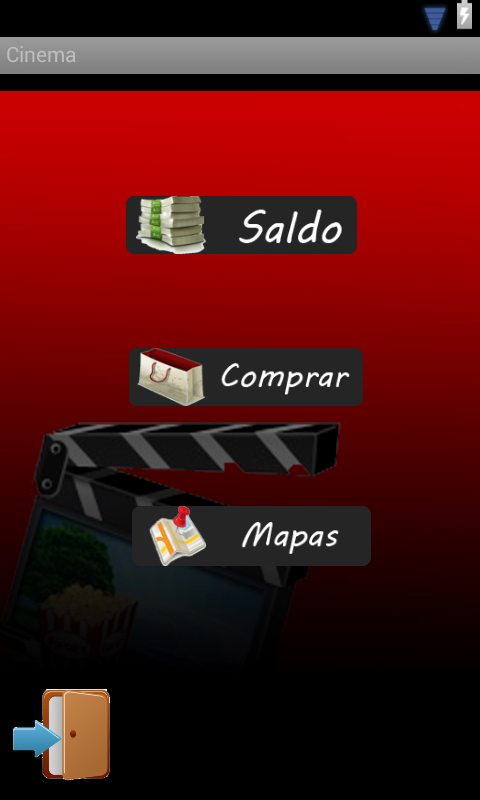
\includegraphics[height=0.8\textheight]{menuprincipal.png}
\end{figure}
\end{frame}

\begin{frame}[allowframbreaks]
\frametitle{Cine actual}
\begin{figure}[h]
\centering
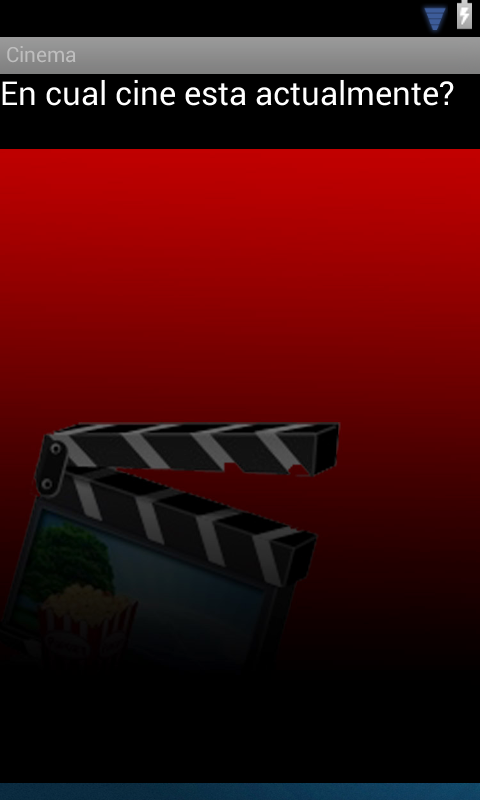
\includegraphics[height=0.8\textheight]{comprar.png}
\end{figure}
\end{frame}

\begin{frame}[allowframbreaks]
\frametitle{Codigo de la Factura}
\begin{figure}[h]
\centering
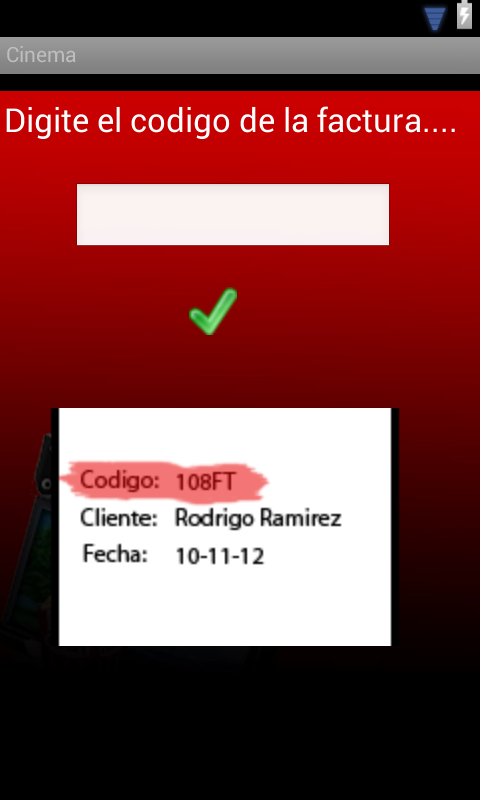
\includegraphics[height=0.8\textheight]{codigofactura.png}
\end{figure}
\end{frame}

\begin{frame}[allowframbreaks]
\frametitle{Menu de comida}
\begin{figure}[h]
\centering
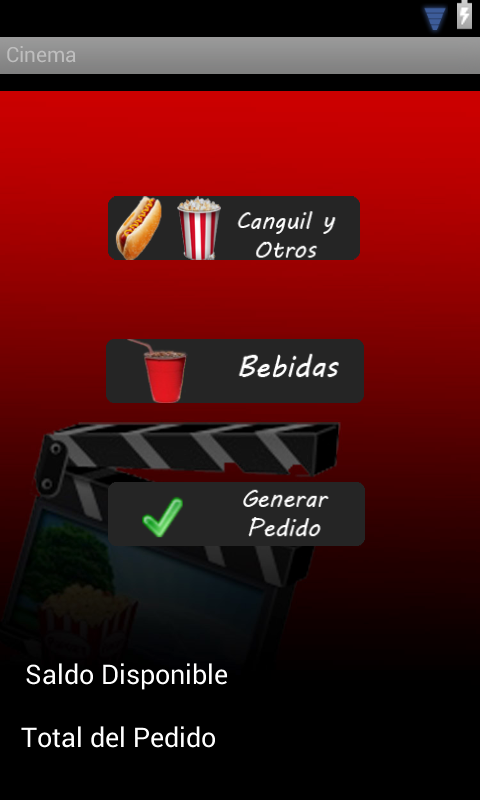
\includegraphics[height=0.8\textheight]{menucompra.png}
\end{figure}
\end{frame}

\begin{frame}[allowframbreaks]
\frametitle{Seleccionar snack}
\begin{figure}[h]
\centering
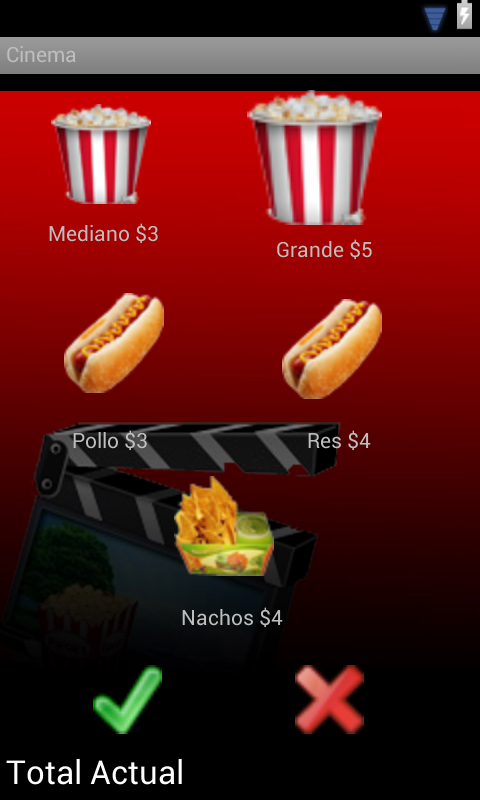
\includegraphics[height=0.8\textheight]{canguil.png}
\end{figure}
\end{frame}

\begin{frame}[allowframbreaks]
\frametitle{Seleccionar bebida}
\begin{figure}[h]
\centering
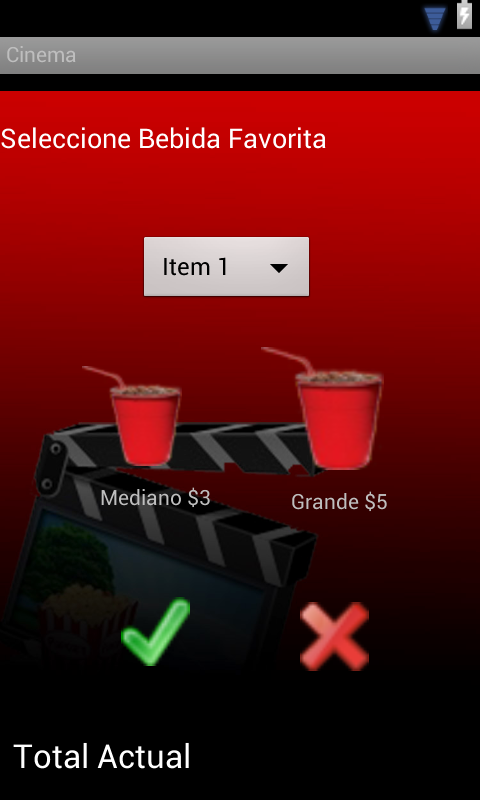
\includegraphics[height=0.8\textheight]{bebidas.png}
\end{figure}
\end{frame}

\begin{frame}[allowframbreaks]
\frametitle{Menu de la comida}
\begin{figure}[h]
\centering
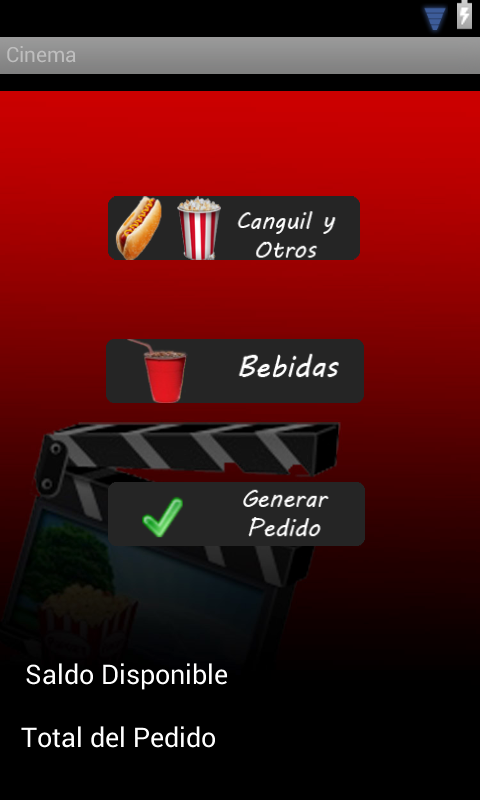
\includegraphics[height=0.8\textheight]{menucompra.png}
\end{figure}
\end{frame}

\begin{frame}[allowframbreaks]
\frametitle{Factura}
\begin{figure}[h]
\centering
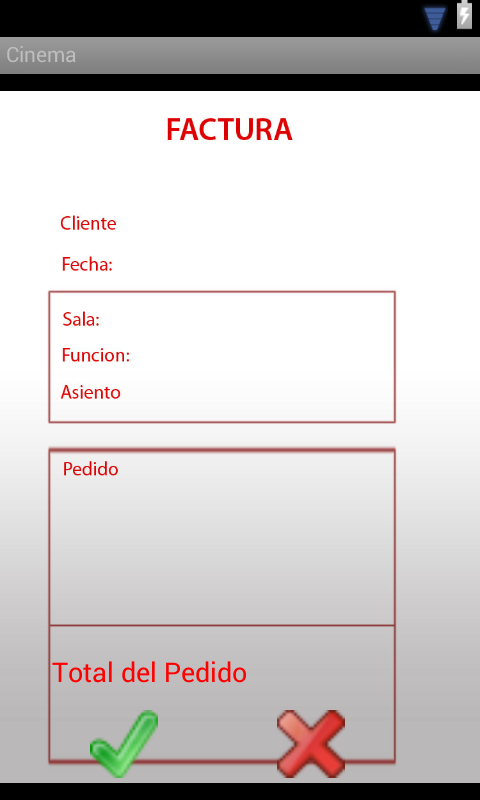
\includegraphics[height=0.8\textheight]{factura.png}
\end{figure}
\end{frame}

\section{Experiencia en desarrollo}
\begin{frame}[allowframebreaks]
\frametitle{Conclusion}
La experiencia final del proyecto fue muy gratificante ya que nos permitio conocer una nueva
plataforma de desarrollo que esta en pleno crecimiento en el mercado mundial en cuestion de
desarrollo de aplicaciones.\\
La experiencia en ciertas partes del codigo fue algo preocupante, debido a que como principiantes
en el desarrollo desconociamos como esta estructurado un proyecto ANDROID.\\
Ademas tuvimos problemas en hacer la conexion a una base de datos externa e interna, las que
finalmente supimos hacerlas
\end{frame}

\begin{frame}[allowframbreaks]
\frametitle{}
Gracias!!!!
\end{frame}


\end{document}